\documentclass[11 pt]{article}

\usepackage[margin=1in]{geometry}

\usepackage{parskip}

\usepackage{amsmath}
\usepackage{amssymb}

\usepackage{graphicx}

\usepackage{array}
\usepackage{booktabs}

\usepackage{microtype}

\usepackage{siunitx}
\usepackage{xspace}

\usepackage{subcaption}

\usepackage{enumerate}

\usepackage{setspace}
% \doublespacing

\usepackage[compact]{titlesec}

% \usepackage[nomarkers, nolists]{endfloat} % places all floats at the end of the document 
% \renewcommand{\efloatseparator}{} % reduce float spacing 


% \usepackage{newtxtext}
% \usepackage{newtxmath}

% Code packages 
	\usepackage[dvipsnames]{xcolor}

	\usepackage{listings}
	\usepackage{color}

	\definecolor{dkgreen}{rgb}{0,0.3,0}
	\definecolor{gray}{rgb}{0.5,0.5,0.5}
	\definecolor{mauve}{rgb}{0.58,0,0.82}	

	\usepackage{inconsolata}

	\lstset{frame=tb,
	  language=Python,
	  aboveskip=3mm,
	  belowskip=3mm,
	  showstringspaces=false,
	  columns=flexible,
	  basicstyle={\small\ttfamily},
	  numbers=none,
	  numberstyle=\tiny\color{gray},
	  keywordstyle=\color{blue},
	  commentstyle=\color{dkgreen},
	  stringstyle=\color{mauve},
	  breaklines=true,
	  breakatwhitespace=true,
	  tabsize=3
	}

	\usepackage{caption}
	\renewcommand{\lstlistingname}{Code}
\makeatletter\@enumdepth1\makeatother


\usepackage{chngcntr}

\usepackage{caption}
\DeclareCaptionFormat{center}{\centerline{#1#2}\\#3}
\captionsetup[figure]{labelsep=period}
\captionsetup[table]{format=center, labelsep=none}
\renewcommand{\tablename}{TABLE}
\renewcommand{\figurename}{Fig.}

% \counterwithin{equation}{pcount}
% \counterwithin{figure}{pcount}
% \counterwithin{table}{pcount}

\usepackage{glossaries}
\makeglossaries
\newacronym{sn}{S$_N$}{Discrete Ordinates}

\newacronym{si}{SI}{Source Iteration}

\newacronym{mhfem}{MHFEM}{Mixed Hybrid Finite Element Method}

% \longnewglossaryentry{computer}
% {
%   name=computer
% }
%   {is a programmable machine that receives input,
%                stores and manipulates data, and provides
%                output in a useful format}

% custom commands 
\newcommand{\SN}{S$_N$\xspace}
\renewcommand{\vec}[1]{\bm{#1}} %vector is bold italic
\newcommand{\vd}{\bm{\cdot}} % slightly bold vector dot
\newcommand{\grad}{\vec{\nabla}} % gradient
\newcommand{\ud}{\mathop{}\!\mathrm{d}} % upright derivative symbol
\newcommand{\pderiv}[2]{\frac{\partial #1}{\partial #2}}
\newcommand{\dderiv}[2]{\frac{\ud #1}{\ud #2}}
\newcommand{\edd}{\langle \mu^2 \rangle} 

\begin{document} % --------------------------------------------------

\newcommand{\HRule}[1]{\rule{\linewidth}{#1}} 	% Horizontal rule

\makeatletter							% Title
\def\printtitle{%						
    {\centering \@title\par}}
\makeatother									

\makeatletter							% Author
\def\printauthor{%					
    {\centering \large \@author}}				
\makeatother							

% --------------------------------------------------------------------
% Metadata (Change this)
% --------------------------------------------------------------------
\title{	\normalsize \textsc{} 	% Subtitle
		 	\\[2.0cm]								% 2cm spacing
			\HRule{0.5pt} \\						% Upper rule
			\LARGE \textbf{\uppercase{Mixed Hybrid Finite Element Eddington Acceleration of Discrete Ordinates Source Iteration}}	% Title
			\HRule{2pt} \\ [0.5cm]		% Lower rule + 0.5cm spacing
			\normalsize \today			% Todays date
		}

\author{
		Samuel S. Olivier\\	
		Texas A\&M University\\	
		Department of Nuclear Engineering\\
        \texttt{smsolivier@tamu.edu} \\
}

\thispagestyle{empty}		% Remove page numbering on this page

\printtitle					% Print the title data as defined above
  	\vfill
\printauthor				% Print the author data as defined above
\newpage

\section{Introduction}
	% Two of the most challenging computational tasks are radiation transport and hydrodynamics. 
	One of the most challenging computational tasks is simulating the interaction of radiation with matter. 
	A full description of a particle in flight includes three spatial variables ($x$,$y$ and $z$), two angular or direction of flight variables ($\mu =$ the cosine of the polar angle and $\gamma =$ the azimuthal angle), one energy variable ($E$) and one time variable ($t$). Numerical solutions require discretizing all seven variables leading to immense systems of algebraic equations. In addition, material properties can lead to vastly different solution behaviors making generalized numerical methods for radiation transport difficult to attain \cite{adams}. 

	% The conservation of mass, momentum and energy in hydrodynamics simulations leads to a hyperbolic system of partial differential equations dependent on the time derivatives of velocity and two state variables. This results in five variables but only three equations leading to the requirement of additional equations to reach problem closure \cite{hydro}. 

	% Radiation transport and hydrodynamics can be combined using operator splitting, where the radiation transport and hydrodynamics 

	Lawrence Livermore National Laboratory (LLNL) is developing a high--order radiation--hydrodynamics code. The hydrodynamics portion is discretized using the \gls{mhfem}, where values are taken to be constant within a cell with discontinuous jumps at both cell edges \cite{mhfem}. \gls{mhfem} is particularly suited for hydrodynamics but not for radiation transport. This work seeks to develop an acceleration scheme capable of robustly reducing the number of iterations in Discrete Ordinates Source Iteration calculations while being compatible with \gls{mhfem} multiphysics.   

\section{Background}
	The steady--state, mono--energetic, isotropically--scattering, fixed--source Linear Boltzmann Equation in planar geometry is: 
		\begin{equation} \label{eq:bte}
			\mu \pderiv{\psi}{x}(x, \mu) + \Sigma_t(x) \psi(x,\mu) = 
			\frac{\Sigma_s(x)}{2} \int_{-1}^{1} \psi(x, \mu') d\mu' + \frac{Q(x)}{2}
		\end{equation}
	where $\mu = \cos\theta$ is the cosine of the angle of flight $\theta$ relative to the $x$--axis, $\Sigma_t(x)$ and $\Sigma_s(x)$ the total and scattering macroscopic cross sections, $Q(x)$ the isotropic fixed--source and $\psi(x, \mu)$ the angular flux \cite{adams}. This is an integro--differential equation due to the placement of the unknown, $\psi(x,\mu)$, under both a derivative and integral.

	The \gls{sn} angular discretization sets $\mu$ to discrete values stipulated by an $N$--point Gauss quadrature rule. The scalar flux, $\phi(x)$, is then 
		\begin{equation} \label{eq:quad}
			\phi(x) = \int_{-1}^1 \psi(x, \mu) \ud\mu 
				\xrightarrow{\text{S}_N} \sum_{n=1}^N w_n \psi_n(x)
		\end{equation}
	where $\psi_n(x) = \psi(x,\mu_n)$ and $w_n$ are the quadrature weights corresponding to each $\mu_n$ \cite{llnl}. The \SN equations are then 
		\begin{equation} \label{eq:sn}
			\mu_n \dderiv{\psi_n}{x}(x) + \Sigma_t(x) \psi_n(x) = 
			\frac{\Sigma_s(x)}{2} \phi(x) + \frac{Q(x)}{2}, \ 1 \leq n \leq N
		\end{equation}
	where $\phi(x)$ is defined by Eq. \ref{eq:quad}. This is now a system of $N$ coupled, ordinary differential equations. 

	The \gls{si} solution method decouples the \gls{sn} equations by lagging the right hand side of Eq. \ref{eq:si}. In other words, 
		\begin{equation} \label{eq:si}
			\mu_n \dderiv{\psi_n^{\ell+1}}{x}(x) + \Sigma_t(x) \psi_n^{\ell+1}(x) = 
			\frac{\Sigma_s(x)}{2} \phi^{\ell}(x) + \frac{Q(x)}{2}, \ 1 \leq n \leq N
		\end{equation}
	where $\psi_n^\ell(x)$ is the solution from the $\ell^\text{th}$ iteration. Equation \ref{eq:si} represents $N$ independent ordinary differential equations. The iteration process begins with an initial guess for the scalar flux, $\phi^0(x)$. Equation \ref{eq:si} is then solved, using $\phi^0(x)$ on the right hand side, for the $\psi_n^1(x)$. $\phi^1(x)$ is then computed using Eq. \ref{eq:quad}.  
	This process is repeated until 
		\begin{equation} \label{eq:converg}
			\frac{\|\phi^{\ell+1}(x) - \phi^{\ell}(x)\|}{\|\phi^{\ell+1}(x)\|} < \epsilon
		\end{equation}
	where $\epsilon$ is a sufficiently small tolerance. 

	If $\phi^0(x) = 0$, then $\phi^\ell(x)$ is the scalar flux of particles that have undergone at most $\ell - 1$ collisions \cite{adams}. Thus, the number of iterations until convergence is directly linked to the number of collisions in a particle's lifetime. Typically, \gls{si} becomes increasingly slow to converge as the ratio of $\Sigma_s$ to $\Sigma_t$ approaches unity and the amount of particle leakage from the system goes to zero. SI is slowest in large, optically thick systems with small losses to absorption. In full radiation transport simulations each iteration could involve solving for hundreds of millions of unknowns. To minimize computational expense, acceleration schemes must be developed to rapidly increase the rate of convergence of \gls{si}. 

	Fortunately, the regime where SI is slow to converge is also the regime where Diffusion Theory is most accurate. A popular method for accelerating SI is \gls{dsa} where each source iteration involves both a transport sweep and a diffusion solve. DSA requires carefully differencing the \gls{sn} and diffusion steps in a consistent manner to prevent instability in highly scattering media with coarse spatial grids \cite{alcouffe,morel}. \gls{dsa} is not applicable in the setting of this presentation due to the incompatibility of MHFEM and \gls{sn} and the increased computational expense of solving consistently differenced diffusion. A new acceleration method is needed that avoids the consistency pitfall of \gls{dsa}. 

\section{Eddington Acceleration}
	The first and second angular moments of Eq. \ref{eq:bte} are 
		\begin{subequations} 
		\begin{equation} \label{eq:zero}
			\dderiv{}{x} J(x) + \Sigma_a(x) \phi(x) = Q(x) 
		\end{equation} 
		\begin{equation} \label{eq:first}
			\frac{\ud}{\ud x} \edd(x) \phi(x) + \Sigma_t(x) J(x) = 0  
		\end{equation}
		\end{subequations}
	where $J(x) = \int_{-1}^{1} \mu \ \psi(x, \mu) \ud \mu$ is the current and 
		\begin{equation} \label{eq:eddington} 
			\edd(x) = \frac{\int_{-1}^1 \mu^2 \psi(x, \mu) \ud \mu}{\int_{-1}^1 \psi(x, \mu) \ud \mu}
			% \xrightarrow{\text{S}_N} \frac{\sum_{n=1}^N \mu_n^2 w_n\psi_n(x)}{\sum_{n=1}^N w_n \psi_n(x)} 
		\end{equation}
	the Eddington factor. In \SN, the Eddington factor is 
		\begin{equation} \label{eq:edd_sn}
			\edd(x) = \frac{\sum_{n=1}^N \mu_n^2 w_n\psi_n(x)}{\sum_{n=1}^N w_n \psi_n(x)}.
		\end{equation}
	Note that no approximations have been made to arrive at Eqs. \ref{eq:zero} and \ref{eq:first}. The Eddington factor is the true angular flux weighted average of $\mu^2$ and therefore Eqs. \ref{eq:zero} and \ref{eq:first} are just as accurate as Eq. \ref{eq:bte}. 

	This formulation is beneficial because Eq. \ref{eq:zero} is a conservative balance equation and---if $\edd(x)$ is known---the moment equations' system of two first--order, ordinary differential equations can be solved directly with well--established methods. However, computing $\edd(x)$ requires already knowing the angular flux. 

	The proposed acceleration scheme is: 
		\begin{enumerate}[1)]
			\item Compute $\psi_n(x)$ with \SN and an arbitrary spatial discretization
			\item Compute $\edd(x)$ with Eq. \ref{eq:edd_sn}
			\item Interpolate $\edd(x)$ onto the MHFEM grid 
			\item Solve the moment equations for $\phi(x)$ with the preconditioned $\edd(x)$ using MHFEM. 
		\end{enumerate}
	This process is one source iteration consisting of an \SN transport step to compute the Eddington factor and an MHFEM acceleration step to compute $\phi(x)$. The scalar flux from the acceleration step is used in the right hand side of Eq. \ref{eq:si} and steps 1--4 are repeated until the acceleration step's $\phi(x)$ converges according to Eq. \ref{eq:converg}.  

	Acceleration occurs because the Eddington factor is a weak function of angular flux. This means that even poor angular flux solutions can accurately approximate the Eddington factor. In addition, the moment equations model the contributions of all scattering events at once, reducing the dependence on source iterations to introduce scattering information. The solution from the acceleration step is then an approximation for the full flux and not the $\ell - 1$ collided flux as it was without acceleration. 

	In addition to acceleration, this scheme allows the \SN equations and moment equations to be solved with different spatial discretizations. \SN can be spatially discretized using normal methods such as \gls{dd} or \gls{ld} while the moment equations can be solved on the same grid as the hydrodynamics. 
	% operator split iteration, computationally economic to use moment equations 

	% This method differs from DSA in that two solutions are generated: one from \SN and one from the moment equations and that the \SN and acceleration steps do not have to be consistently differenced. The solution of the moment equations will be used because the moment equations are conservative while \SN is not. 

\section{Transport Step}

%!TEX root = ./writeup.tex

\section{Diamond Differenced Discrete Ordinates}
	The Diamond Differenced (DD) \SN equations corresponding to Eq. \ref{eq:sn} are 
		\begin{equation} \label{eq:dd}
			\frac{\mu_n}{h_i}\left(\psi_{n,i+1/2} - \psi_{n,i-1/2}\right)
				+ \Sigma_{t,i} \psi_{n,i} = \frac{\Sigma_{s,i}}{2}\sum_{n'=1}^N \psi_{n',i}w_{n'}
				+ \frac{Q_i}{2} , \ 1 \leq n \leq N, \ 1 \leq i \leq I
		\end{equation}
	where $\psi_{n,i\pm1/2} = \psi_n(x_{i\pm1/2})$ is the cell edge angular flux and $\Sigma_{t,i} = \Sigma_t(x_i)$, $\Sigma_{s,i} = \Sigma_s(x_i)$ and $Q_i = Q(x_i)$ the cell averaged total cross section, scattering cross section and fixed source. The $x_{i\pm1/2}$ are the cell edge locations of cell $i$ of cell width $h = x_{i+1/2} - x_{i-1/2}$. In DD, the cell centered angular flux is taken to be the average of the adjacent cell edge angular fluxes: 
		\begin{equation} \label{eq:auxDD}
			\psi_{n,i} = \frac{1}{2} \left(\psi_{n,i+1/2} + \psi_{n,i-1/2}\right).
		\end{equation}
	Using this result for the scattering term yields
		\begin{align}
			\frac{\Sigma_{s,i}}{2}\sum_{n'=1}^N \psi_{n',i}w_{n'} &= 
			\frac{\Sigma_{s,i}}{2}\sum_{n'=1}^N 
				\frac{1}{2} \left(\psi_{n,i+1/2} + \psi_{n,i-1/2}\right) w_{n'} \\
			&= \frac{\Sigma_{s,i}}{4} \left(\phi_{i-1/2} + \phi_{i+1/2}\right)
		\end{align}
	In SI, the scattering term is lagged: 
		\begin{equation} \label{eq:DDSN}
			\frac{\mu_n}{h_i}\left(\psi_{n,i+1/2}^{\ell+1} - \psi_{n,i-1/2}^{\ell+1}\right)
				+ \Sigma_{t,i} \psi_{n,i}^{\ell+1} = 
				\frac{\Sigma_{s,i}}{4} \left(\phi_{i-1/2}^\ell + \phi_{i+1/2}^\ell\right)
				+ \frac{Q_i}{2}, \ 
			1 \leq n \leq N, \ 1 \leq i \leq I
		\end{equation}
	Solving for $\psi_{n,j\pm1/2}^{\ell+1}$ yields  
		\begin{subequations}
			\begin{equation} \label{eq:psiplus}
				\psi_{n,j+1/2}^{\ell+1} = 
				\frac{
				\frac{\Sigma_s}{2}h_i \left(\phi_{i-1/2}^\ell + \phi_{i+1/2}^\ell\right)
				+ Q_i h_i - \left(\Sigma_t h_i - 2\mu_n\right) \psi_{n,i-1/2}^{\ell+1}
				}
				{
				\Sigma_t h_i + 2\mu_n 
				}, \ \mu_n > 0 
			\end{equation}
			\begin{equation} \label{eq:psiminus}
				\psi_{n,j-1/2}^{\ell+1} = 
				\frac{
				\frac{\Sigma_s}{2}h_i \left(\phi_{i-1/2}^\ell + \phi_{i+1/2}^\ell\right)
				+ Q_i h_i - 
					\left(\Sigma_t h_i - 2|\mu_n|\right) \psi_{n,i+1/2}^{\ell+1}
				}
				{
				\Sigma_t h_i + 2|\mu_n| 
				}, \ \mu_n < 0 
			\end{equation}
		\end{subequations}
	Equation \ref{eq:psiplus} specifies the flux exiting the right side of cell $i$ given the flux that entered through the left side while Eq. \ref{eq:psiminus} specifies the flux exiting the left side of cell $i$ given the flux that entered through the right side. 

	By specifying boundary conditions for $\psi_{n,1/2}^{\ell+1}$ for $\mu_n>0$ and $\psi_{n,I+1/2}^{\ell+1}$ for $\mu<0$, Eqs. \ref{eq:psiplus} and \ref{eq:psiminus} can be solved non-iteratively. The boundary conditions for a vacuum left boundary and reflecting right boundary are 
		\begin{subequations}
		\begin{equation} \label{eq:leftBC}
			\psi_{n,1/2}^{\ell+1} = 0, \ \mu_n > 0
		\end{equation}
		\begin{equation} \label{eq:rightBC}
			\psi_{n,I+1/2}^{\ell+1} = \psi_{m,I+1/2}^{\ell+1}, \ \mu_n = -\mu_m.
		\end{equation}
		\end{subequations}

	Using Eq. \ref{eq:leftBC}, the flux exiting the right side of cell $i=1$, $\psi_{n,3/2}^{\ell+1}$, can be found through Eq. \ref{eq:psiplus}. This exiting flux is then the flux entering cell $i=2$ allowing for the determination of $\psi_{n,5/2}^{\ell+1}$. This process of using the result from the previous cell is repeated until $i=I$. At this point all rightward ($\mu>0$) moving flux has been determined for all cells $1 \leq i \leq I$. 

	The reflecting boundary condition, Eq. \ref{eq:rightBC}, can now be applied. This sets the incoming flux on the right side of cell $i=I$. Equation \ref{eq:psiminus} then determines the exiting flux through the left side, $\psi_{n,I-1/2}^{\ell+1}$. Working backward from cell $i=I$, $\psi_{n,I-3/2}^{\ell+1}, \psi_{n,I-5/2}, \dots, \psi_{n,1/2}^{\ell+1}$ for $\mu_n < 0$ can be found. 

	This process of propagating the solution from left to right for $\mu_n > 0$ and then from right to left for $\mu_n < 0$ is known as a transport sweep. At the end of the sweep, new cell edge scalar flux values $\phi_{i\pm1/2}^{\ell+1}$ are generated through 
		\begin{equation}
			\phi_{i\pm1/2}^{\ell+1} = \sum_{n=1}^N \psi_{n,i\pm1/2}^{\ell+1} w_n. 
		\end{equation}
	A new sweep is then conducted using $\phi_{i\pm1/2}^{\ell+1}$. This process is repeated until the stop criterion of 
		\begin{equation}
			\frac{
			\sum_{i=0}^{I} \left(\phi_{i+1/2}^{\ell+1} - \phi_{i+1/2}^\ell\right)^2
			}{
			\sum_{i=0}^{I} \left(\phi_{i+1/2}^{\ell+1}\right)^2
			}
			< \epsilon
		\end{equation}
	is met. 

\subsection{Linear Discontinuous Galerkin Discrete Ordinates}

%!TEX root = ./writeup.tex

\newcommand{\bl}{B_{L,i}(x)}
\newcommand{\br}{B_{R,i}(x)}
\newcommand{\jil}{J_{i,L}}
\newcommand{\jir}{J_{i,R}}
\newcommand{\eddphi}[1]{\edd_{#1}\phi_{#1}}
\newcommand{\alphai}[2]{\frac{#1}{\Sigma_{t,#2}h_{#2}}}

\section{Mixed Hybrid Finite Element Method Acceleration}

The \gls{mhfem} as applied to Eqs. \ref{eq:zero} and \ref{eq:first} uses the following basis functions:
	\begin{subequations}
	\begin{equation} \label{mhfem:BL}
		\bl = \begin{cases}
			\frac{x_{i+1/2} - x}{x_{i+1/2} - x_{i-1/2}}, \ x \in [x_{i-1/2}, x_{i+1/2}] \\ 
			0, \ \text{otherwise}
		\end{cases}
	\end{equation}
	\begin{equation} \label{mhfem:BR}
		\br = \begin{cases}
			\frac{x - x_{i-1/2}}{x_{i+1/2} - x_{i-1/2}}, \ x \in [x_{i-1/2}, x_{i+1/2}] \\ 
			0, \ \text{otherwise}
		\end{cases}. 
	\end{equation}
	\end{subequations}
The scalar flux is constant within a cell with discontinuous jumps at the cell edges. In other words, 
	\begin{equation} \label{mhfem:flux}
		\phi_i(x) = \begin{cases}
			\phi_i, \ x \in (x_{i-1/2}, x_{i+1/2}) \\ 
			\phi_{i\pm 1/2}, x = x_{i\pm1/2} \\ 
			0, \ \text{otherwise}
		\end{cases} 
	\end{equation}
with 
	\begin{equation} \label{mhfem:sumphi}
		\phi(x) = \sum_{i=1}^I \phi_i(x). 
	\end{equation}
The Eddington factor will be interpolated onto the same grid as the scalar flux so that cell edge and cell center values will be available.  

The current, $J(x)$, is a linear function defined by 
	\begin{equation} \label{mhfem:J}
		J(x) = \sum_{i=1}^I \jil \bl + \jir \br
	\end{equation} 
where $\jil$ and $\jir$ are the current on the left and right edges of the cell. 

There are five unknowns in every cell $\phi_{i-1/2}$, $\phi_{i}$, $\phi_{i+1/2}$, $\jil$, and $\jir$. Thus, five equations are needed. The first equation is obtained by integrating Eq. \ref{eq:zero} over cell $i$
	\begin{equation} \label{mhfem:balance}
		\jir - \jil + \Sigma_{a,i} \phi_i h_i = Q_i h_i. 
	\end{equation}
Equations for the cell edge current, $\jil$ and $\jir$, are found by multiplying Eq. \ref{eq:first} by $\bl$ and $\br$ and integrating over cell $i$. This yields 
	\begin{subequations}
	\begin{equation}
		\int_{x_{i-1/2}}^{x_{i+1/2}} \bl \dderiv{}{x} \edd(x) \phi(x) + \bl \Sigma_t(x) J(x) \ud x
	\end{equation}
	\begin{equation}
		\int_{x_{i-1/2}}^{x_{i+1/2}} \br \dderiv{}{x} \edd(x) \phi(x) + \br \Sigma_t(x) J(x) \ud x
	\end{equation}
	\end{subequations}
Integrating by parts produces 
	\begin{subequations}
	\begin{equation} \label{mhfem:half1}
		-\edd_{i-1/2}\phi_{i-1/2} + \edd_i \phi_i + \Sigma_{t,i} h_i \left(\frac{\jil}{3}
			+ \frac{\jir}{6} \right) = 0
	\end{equation}
	\begin{equation} \label{mhfem:half2}
		\edd_{i+1/2}\phi_{i+1/2} - \edd_i \phi_i + \Sigma_{t,i}h_i \left(\frac{\jil}{6} + \frac{\jir}{3}\right) = 0.
	\end{equation}
	\end{subequations}
Eliminating $\jil$ from Eq. \ref{mhfem:half1} and $\jir$ from Eq. \ref{mhfem:half2} results in the second and third equations
	\begin{equation} \label{mhfem:jir_f}
		\jir = \frac{-2}{\Sigma_{t,i}h_i} \left[ \eddphi{i-1/2} - 3\eddphi{i} + 2\eddphi{i+1/2} \right]
	\end{equation}
	\begin{equation} \label{mhfem:jil_f}
		\jil = \frac{-2}{\Sigma_{t,i} h_i} \left[ -2 \eddphi{i-1/2} + 3\eddphi{i} - \eddphi{i+1/2}\right]
	\end{equation}

Continuity of current is ensured through enforcing 
	\begin{equation}
		\jir = J_{i+1,L}
	\end{equation}
and 
	\begin{equation}
		\jil = J_{i-1,R}. 
	\end{equation}
Applying these two conditions yields the fourth and fifth equations:
	\begin{equation}
		\begin{aligned}
		\alphai{-2}{i} \eddphi{i-1/2} &+ \alphai{6}{i} \eddphi{i} - 4 \left(
			\frac{1}{\Sigma_{t,i}h_i} + \frac{1}{\Sigma_{t,i+1}h_{i+1}}\right)\eddphi{i+1/2} \\
		&+ \alphai{6}{i+1}\eddphi{i+1} - \alphai{2}{i+1}\eddphi{i+3/2} = 0
		\end{aligned}
	\end{equation}
	\begin{equation}
		\begin{aligned}
		\alphai{-2}{i-1} \eddphi{i-3/2} &+ \alphai{6}{i-1} \eddphi{i-1} - 4 \left(
			\frac{1}{\Sigma_{t,i-1}h_{i-1}} + \frac{1}{\Sigma_{t,i}h_{i}}\right)\eddphi{i-1/2} \\
		&+ \alphai{6}{i}\eddphi{i} - \alphai{2}{i}\eddphi{i+1/2} = 0
		\end{aligned}
	\end{equation}

Equations \ref{mhfem:jir_f} and \ref{mhfem:jil_f} can be subbed into Eq. \ref{mhfem:balance} to reduce the system to three equations, three unknowns. The resulting system is 
	\begin{subequations}
		\begin{equation}
			\alphai{-6}{i}\eddphi{i-1/2} + \left(\Sigma_{a,i}h_i + \alphai{12}{i}\edd_i\right) \phi_i - \alphai{6}{i}\eddphi{i+1/2} = Q_i h_i
		\end{equation}
		\begin{equation}
			\begin{aligned}
			\alphai{-2}{i} \eddphi{i-1/2} &+ \alphai{6}{i} \eddphi{i} - 4 \left(
				\frac{1}{\Sigma_{t,i}h_i} + \frac{1}{\Sigma_{t,i+1}h_{i+1}}\right)\eddphi{i+1/2} \\
			&+ \alphai{6}{i+1}\eddphi{i+1} - \alphai{2}{i+1}\eddphi{i+3/2} = 0
			\end{aligned}
		\end{equation}
		\begin{equation}
			\begin{aligned}
			\alphai{-2}{i-1} \eddphi{i-3/2} &+ \alphai{6}{i-1} \eddphi{i-1} - 4 \left(
				\frac{1}{\Sigma_{t,i-1}h_{i-1}} + \frac{1}{\Sigma_{t,i}h_{i}}\right)\eddphi{i-1/2} \\
			&+ \alphai{6}{i}\eddphi{i} - \alphai{2}{i}\eddphi{i+1/2} = 0
			\end{aligned}
		\end{equation}
	\end{subequations}

The Marshak boundary condition is 
	\begin{equation}
		\phi(x) - 2J(x) = 0. 
	\end{equation}
Applied to the left edge of the domain, the equations for cell $i=1$ are 
	\begin{equation}
		\phi_{1/2} - 2\jil = 0
	\end{equation}
Apply a reflecting boundary on the right edge 
	\begin{equation}
		J(x_{N+1/2}) = J_{N,R} = 0. 
	\end{equation}



\section{Results}
	As a proof of concept for Eddington acceleration, a \gls{dd} \gls{sn} code was created along with an \gls{mhfem} solver for Eqs. \ref{eq:zero} and \ref{eq:first}. The test problem of steady--state, one--group, isotropically--scattering, fixed--source radiation transport in slab geometry with a reflecting left boundary and vacuum right boundary was used to compare unaccelerated, Eddington accelerated, and DSA S$_8$ SI with 100 spatial cells. 

	\begin{figure} % replace 't' with 'b' to force it to be on the bottom
		\centering
		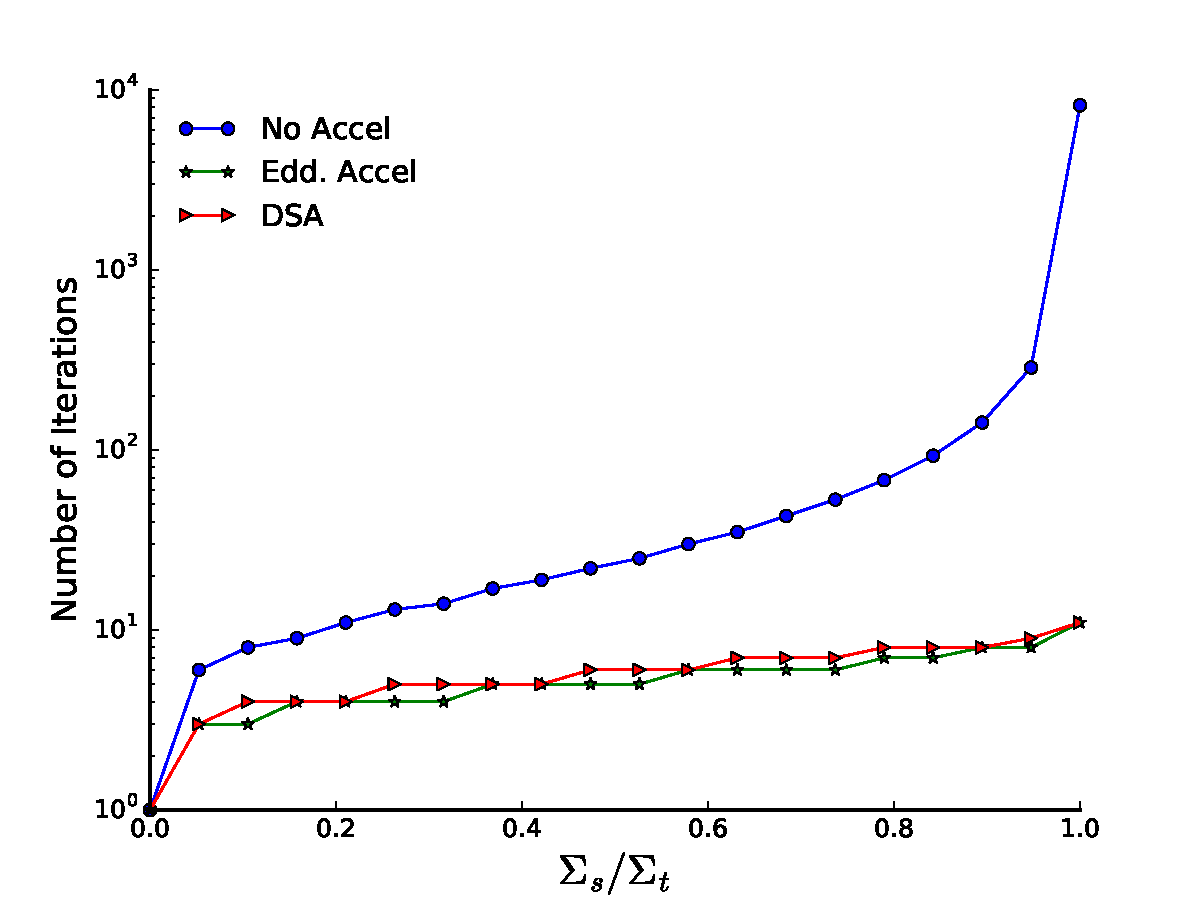
\includegraphics[width=5in]{accel.pdf}
		\caption{A comparison of the number of iterations until convergence for unaccelerated, Eddington accelerated, and DSA S$_8$ SI. }
		\label{fig:comparison}
	\end{figure}

	Figure \ref{fig:comparison} shows the number of iterations until the convergence criterion in  Eq. \ref{eq:converg} was met with $\epsilon = \num{1e-6}$ for varying ratios of $\Sigma_s$ to $\Sigma_t$. Aside from $\Sigma_s/\Sigma_t = 0$ where acceleration is not possible, the ratio of unaccelerated to Eddington accelerated iterations ranges between 2.5 and 750. This suggests that acceleration is occurring and that Eddington acceleration does not just do twice the amount of work in each iteration. 

	Figure \ref{fig:conv_si} shows the unaccelerated convergence criterion 
		\begin{equation}
			\frac{\|f^{\ell+1} - f^{\ell}\|}{\|f^{\ell+1}\|}
		\end{equation}
	as a function of iteration number for $f = \phi(x)$ and $f = \edd(x)$. The large drop in the convergence criterion between the first and second iterations supports the claim that $\edd(x)$ is a weak function of angular flux as it quickly converges despite a less convergent angular flux. When compared to Fig. \ref{fig:conv_edd}, a plot of the convergence criterion versus number of iterations for Eddington accelerated S$_8$, it is clear that Eddington acceleration transfers the fast rate of convergence of $\edd(x)$ to $\phi(x)$. 

	\begin{figure}
		\centering
		\begin{subfigure}{.49\textwidth} 
			\centering
			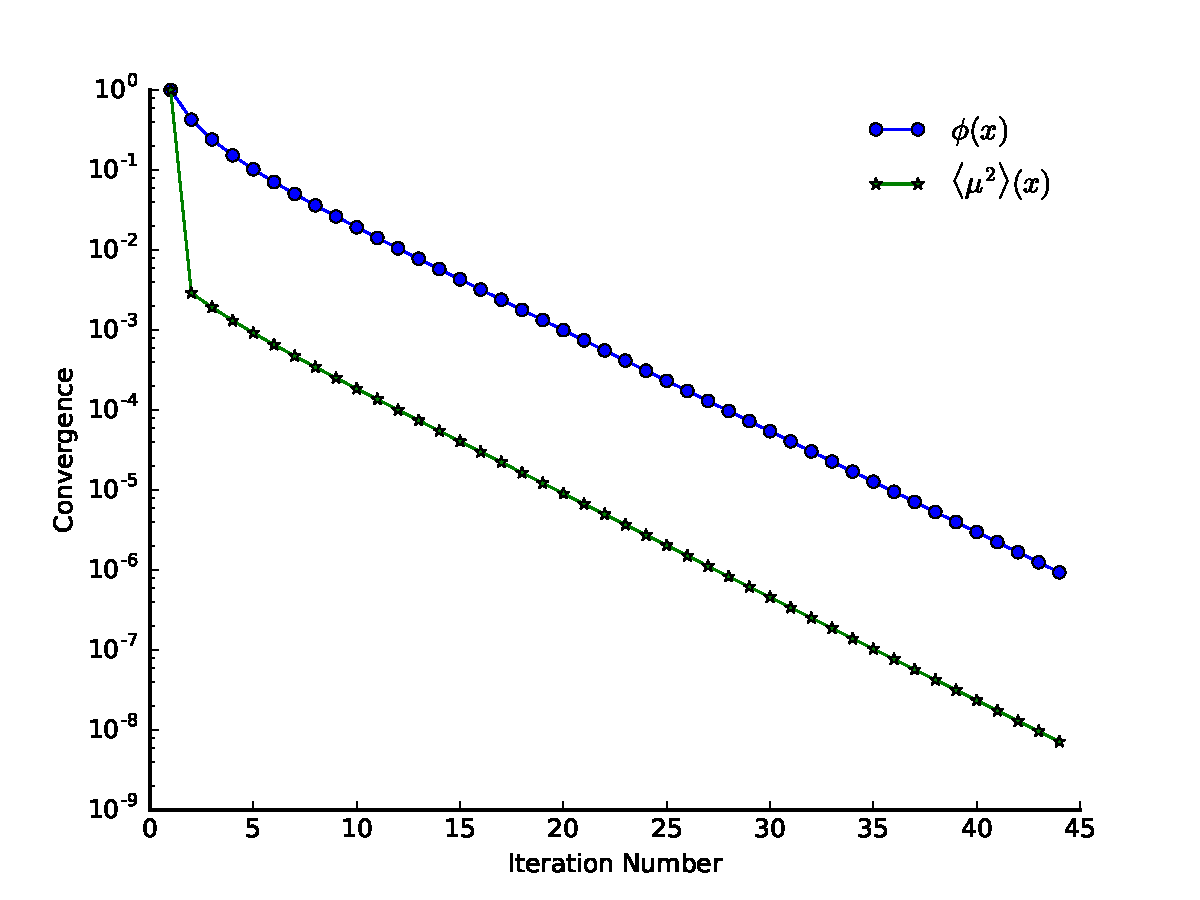
\includegraphics[width=\textwidth]{eddCon_si.pdf}
			\caption{}
			\label{fig:conv_si}
		\end{subfigure}
		\begin{subfigure}{.49\textwidth}
			\centering
			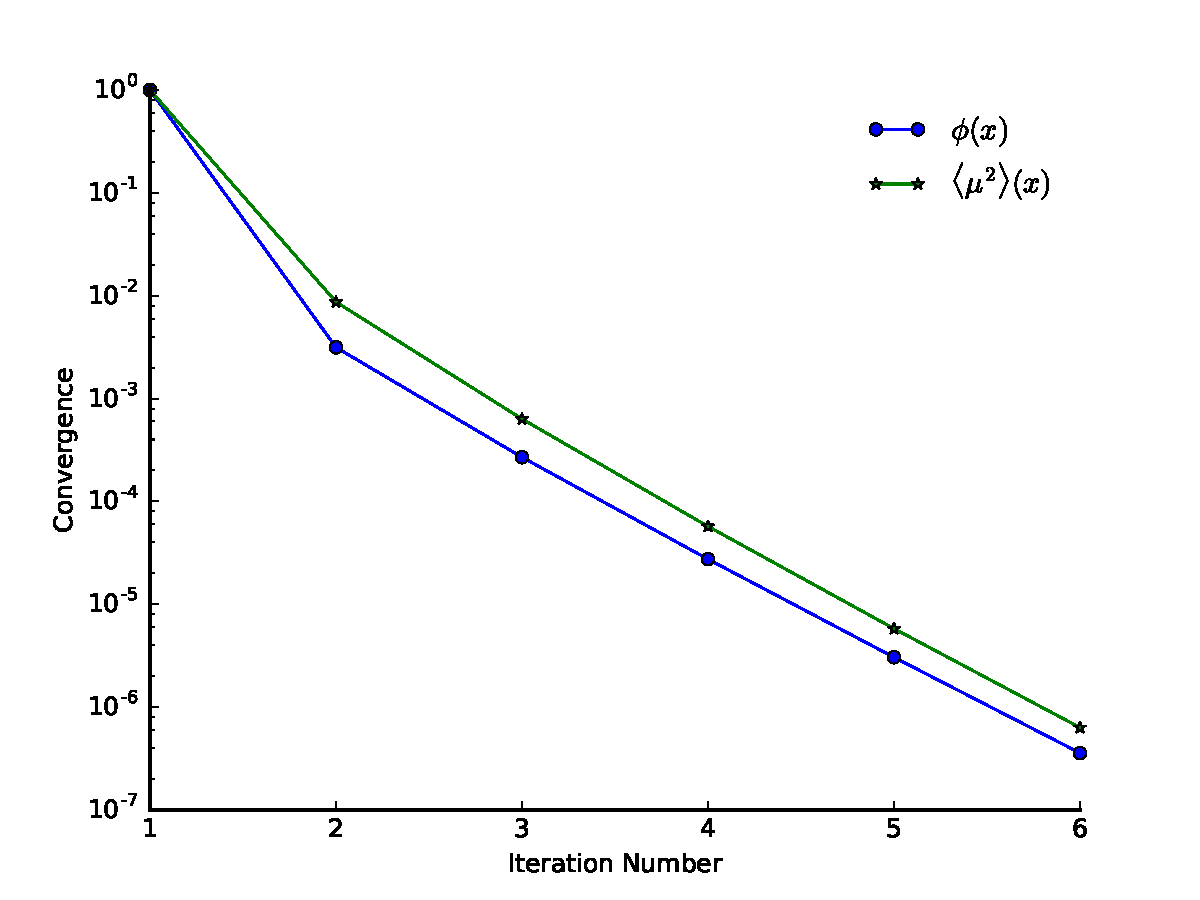
\includegraphics[width=\textwidth]{eddCon_mu.pdf}
			\caption{}
			\label{fig:conv_edd}
		\end{subfigure}
		\caption{The convergence rate of $\phi(x)$ compared to $\edd(x)$ for (a) unaccelerated and (b) Eddington accelerated S$_8$. }
	\end{figure}

	% add convergence rate of phi v edd 
	% include discussion on acceleration v just doing 2 times as much work. ie actual acceleration is happening 

\section{Conclusions}
	The proposed acceleration scheme successfully accelerated S$_8$ source iteration calculations in slab geometry for a wide range of $\Sigma_s/\Sigma_t$. In the pure scattering regime ($\Sigma_s = \Sigma_t$), source iteration was accelerated by a factor of 750. This scheme is especially suited for multiphysics applications because the transport and acceleration steps do not need to be consistently differenced. In addition, the acceleration step produces a conservative solution that is computationally inexpensive compared to a transport sweep. Future work that will also be presented is the application of Eddington acceleration to Linear Discontinuous Galerkin discretized \SN. 

% \clearpage
\bibliographystyle{ans}
\bibliography{bibliography} 

\printglossaries
\end{document} % --------------------------------------------------